\documentclass[a5paper, twoside]{article}

%\usepackage{showframe}

\usepackage[flowers]{../../template}
\usetikzlibrary{tikzmark}
\usetikzlibrary{fit}

\geometry{
%  showframe,
  a5paper, 
  total={124.5mm, 165mm}, 
  top=20mm, 
  marginpar={0mm},
  left={12mm},
  %right={26mm},
  headsep=5mm
}

\pdfcompresslevel=0


\renewcommand{\contentsname}{Spis rozmaitości treściowalnych}

\usepackage{titlesec}
\usepackage[dotinlabels]{titletoc}
\titleformat{\section}[hang]{\color{purple}\sffamily\bfseries\Large}{\color{purple}Wykład }{0.2em}{}
\titlespacing*{\section}{0pt}{2\baselineskip}{1.25\baselineskip}
\titleformat{\subsection}[hang]{\color{purple}\sffamily\bfseries\large}{\color{purple}\thesubsection}{0.4em}{}
\titlespacing*{\subsection}{2em}{1\baselineskip}{1\baselineskip}

\makeatletter %only needed in preamble
\renewcommand\Large{\@setfontsize\Large{12pt}{9}}
\renewcommand\large{\@setfontsize\large{10pt}{9}}
\renewcommand\scriptsize{\@setfontsize\scriptsize{5pt}{5}}
\renewcommand\small{\@setfontsize\small{6pt}{6}}
\makeatother

\fancyhead[LE, RO]{\rightmark}

\setheader{Algebra homologiczna}
\setfoot{Dymary}

\fancyfoot[LE, RO]{\color{black!20}\scalefont{0.8} }%Weronika Jakimowicz}

\title{Algebra homologiczna}
\author{}
\date{Zima 2023-24}

\begin{document}
\scalefont{0.8}

\maketitle
\thispagestyle{empty} 
\newpage

\tableofcontents
\thispagestyle{empty}
\newpage

\pagestyle{fancy}

\section{04.10.23 : Wstęp}

\subsection{Co to kategoria}

Rozważmy układ danych $\mathbf{C}$ zawierający:
  \begin{itemize}
    \item klasę \acc{obiektów} $\ob\mathbf{C}$
    \item dla dowolnej pary $X,Y\in \ob\mathbf{C}$ zbiór $Hom_{\mathbf{C}}(X, Y)$, którego elementy nazywany \acc{morfizmami} i zapisujemy $\phi:X\to Y$ lub $X\xrightarrow{\phi} Y$
    \item kolekcję odwzorowań, zwanych \acc{złożeniami}, dla wszystkich $X,Y,Z\in \ob\mathbf{C}$ takich, że
      \begin{center}\begin{tikzcd}[row sep=tiny, column sep=small]%, /tikz/column 2/.style={column sep=1pt}, /tikz/column 1/.style={column sep=1pt}]
        Hom_{\mathbf{C}}(X, Y)\times Hom_{\mathbf{C}}(Y, Z)\arrow[r] & Hom_{\mathbf{C}}(X, Z)\\ 
        (\;\phi,\quad\psi\;)\arrow[u, sloped, phantom, "\in", yshift=12pt]\arrow[u, phantom, sloped, "\in", yshift=-12pt]\arrow[r, mapsto] & \psi\circ\phi\arrow[u, phantom, sloped, "\in"]
      \end{tikzcd}\end{center}
  \end{itemize}

\begin{definition}[kategoria (mała)]
  Układ danych $\mathbf{C}$ jak wyżej nazywamy \buff{kategorią}, jeśli spełnione są następujące warunki:
  \begin{enumerate}
    \item Zbiory $Hom_{\mathbf{C}}(X, Y)$ dla $X,Y\in\ob\mathbf{C}$ są parami rozłączne (tzn. morfizmy mają dobrze określone dziedziny i przeciwdziedziny).
    \item Dla każdego $A\in\ob\mathbf{C}$ istnieje $Id_A\in Hom_{\mathbf{C}}(A, A)$ takie, że $\phi\circ Id_A=\phi$ oraz $Id_A\circ\psi=\psi$.
    \item Złożenie morfizmów jest łączne, tzn. dla morfizmów
      \begin{center}\begin{tikzcd}
        X\arrow[r, "\phi"] & Y\arrow[r, "\psi"] & Z\arrow[r, "\eta"] & W
      \end{tikzcd}\end{center}
      zawsze zachodzi równość $(\eta\psi)\phi=\eta(\psi\phi)$.
  \end{enumerate}

  Dodatkowo, jeśli $\ob\mathbf{C}$ jest zbiorem, to $\mathbf{C}$ nazywamy \acc{małą kategorią}.
\end{definition}

\begin{example}
\item Kategorię wszystkich pierścieni wektorowych nad ciałem $K$ oznaczamy $\mathbf{Vect}_k$. Jeśli interesują nas przestrzenie tylko skończonego wymiaru, to istnieje kategoria $\mathbf{Vect}_K^{fin}$ przestrzeni wektorowych skończenie wymiarowych. 

  Obiektami obu tych kategorii są przestrzenie liniowe (skończonego wymiaru), a morfizmami są przekształcenia liniowe między nimi.
\item Wszystkie zbiory wraz z funkcjami między nimi jako morfizmami tworzą kategorią $\mathbf{Set}$ zbiorów.
\item Jeśli rozważamy jako obiekty tylko zbiory z określonym dobrym porządkiem, to morfizmami mogą być funkcje słabo monotoniczne. Taką kategorię oznaczamy $\mathbf{Set}_\leq$.
\item Kategoria wszystkich grup wraz z homomorfizmami jako morfizmami jest oznaczana $\mathbf{Grp}$, natomiast kategoria, której obiekty to tylko grupy abelowe jest oznaczana $\mathbf{Ab}$.
\item Pojedyncza grupa $G$ może tworzyć sama w sobie jednoobiektową kategorię $\mathbf{C}_G$ taką, że
  \begin{itemize}
    \item $\ob\mathbf{C}_G=\{\star\}$
    \item $Hom_{\mathbf{C}_G}(\star,\star)=G$, a złożenia działa jak mnożenie elementów $G$.
    \end{itemize}
\item Dla dowolnego pierścienia $R$ istnieje kategoria, której obiektami są (lewe) $R$-moduły, a morfizmami są homomorfizmy między tymi modułami. Oznaczamy to $R-\mathbf{mod}$.
\item Wszystkie przestrzenie topologiczne wraz z odwzorowaniami ciągłymi nazywamy kategorią przestrzeni topologicznych $\mathbf{Top}$.
\item Wszystkie gładkie rozmaitości są obiektami kategorii $\mathbf{Diff}$, a morfizmy to gładkie odwzorowania między rozmaitościami.
\item Kategoria $\mathbf{Rep}_{G,K}$ posiada jako obiekty reprezentacje grupy $G$ na przestrzeniach liniowych nad $K$, a jako morfizmy wszystkie przekształcenia $G$-ekwiwariantne.
\end{example}

\subsection{Kompleksy}

\begin{definition}[kompleksy łańcuchowe (grup abelowych)]
  Jeśli ciąg (grup abelowych) $A_\cdot$
  \begin{center}\begin{tikzcd}
    ...\arrow[r] & A_0\arrow[r, "d_0"] & A_1\arrow[r, "d_1"] & A_2 \arrow[r, "d_2"] & ...
  \end{tikzcd}\end{center}
  jest taki, że dla każdego $n\Z$ (dopuszczamy ujemne indeksy) złożenie $d_{n+1}\circ d_n=0$, to nazywamy go \buff{kompleksem łańcuchowym}.
\end{definition}

Możemy rozważać kategorię, której obiektami są kompleksy łańcuchowe obiektów z jednej kategorii $\mathbf{C}$, np. grup abelowych. Morfizmem między kompleksem $A_\cdot$ a kompleksem $B_\cdot$ nazwiemy wówczas ciąg homomorfizmów $\phi_i\in Hom_{\mathbf{C}}(A_i,B_i)$ taki, że w diagramie
  \begin{center}\begin{tikzcd}
    ...\arrow[r] & A_0\arrow[r, "d^A_0"]\arrow[d, "\phi_0" left] & A_1\arrow[r, "d^A_1"]\arrow[d, "\phi_1"] & A_2 \arrow[r, "d^A_2"]\arrow[d, "\phi_2"] & ... \\
    ...\arrow[r] & B_0\arrow[r, "d^B_0"] & B_1\arrow[r, "d^B_1"] & B_2 \arrow[r, "d^B_2"] & ...
  \end{tikzcd}\end{center}
każdy prostokąt komutuje, tzn.
$$d^B_n\circ\phi_n=\phi_{n+1}\circ d_{n}^A$$
dla każdego $n$.

\subsection{Funktory kowariantne i kontrawariantne}

\begin{definition}[funktor]
  \buff{Funktorem} z kategorii $\mathbf{C}$ w kategorię $\mathbf{D}$ nazywamy dwa przyporządkowania: między obiektami tych kategorii i między morfizmami takie, że:
  \begin{itemize}
    \item $\ob\mathbf{C}\ni X\mapsto F(X)\in\ob\mathbf{D}$
    \item dla każdej pary $X,Y\in\ob\mathbf{C}$ odwzorowanie
      $$Hom_{\mathbf{C}}(X, Y)\ni \phi\mapsto F(\phi)\in Hom_{\mathbf{D}}(F(X),F(Y))$$
      zachowuje składanie morfizmów, tzn. $F(\phi\circ\psi)=F(\phi)\circ F(\psi)$.
  \end{itemize}

  Takie przyporządkowania między kategoriami nazywa się też, bardziej precyzyjnie, \acc{funktorami kowariantnymi}.
\end{definition}

\begin{example}
\item Funktor $F:\mathbf{Set}\to \mathbf{Vect}_K$ zdefiniujmy tak, że dowolny $X\in\ob\mathbf{Set}$ przechodzi ma przestrzeń wektorową nad ciałem $K$ o bazie $X$, tzn.:
  $$F(X)=\left\{\sum_{x\in X} a_xx\;:\;\alpha_x\in K\text{, tylko skończenie wiele }\neq0\right\}$$
\end{example}

\begin{definition}[kategoria dualna]
  Dla kategorii $\mathbf{C}$ możemy zdefiniować nową kategorię, $\mathbf{C}^{op}$ w której każdy morfizm $\phi^{op}\in Hom_{\mathbf{C}^{op}}(Y, X)$ zostaje odwrócony:
  \begin{center}\begin{tikzcd}
    X\arrow[r, bend left=20, "\phi"] & Y\arrow[l, bend left=20, "\phi^{op}"]
  \end{tikzcd}\end{center}
  Wtedy $\ob\mathbf{C}^{op}$ to obiekty dualne do elementów znajdujących się w $\ob\mathbf{C}$. Tak zdefiniowaną kategorię $\mathbf{C}^{op}$ nazywamy \buff{kategorią dualną}.
\end{definition}

\begin{example}
\item Kategoria dualna do kategorii przestrzeni liniowych $\mathbf{Vect}_K^{op}$ jest kategorią, której obiekty to przestrzenie sprzężone, $V^*\in\ob\mathbf{Vect}^{op}_K$, zawierające funkcjonały liniowe $V\to K$. Każdy morfizm $\phi:V\to W$ w $\mathbf{Vect}_K$ indukuje wówczas odwzorowanie $\phi^*:W^*\to V^*$ takie, że dla $f\in W^*$ mamy $\phi^*(f)=f\circ\phi:V\to W\to K$.

  Kojarzenie funkcjonału $\phi^*\in V^*$ z elementem $v\in V$ jest czasem oznaczane przez $\langle \phi, v\rangle=\phi(v)$.
\end{example}

\begin{definition}[funktor kontrawariantny]
  Funktor (kowariantny) z kategorii $\mathbf{C}^{op}$ do kategorii $\mathbf{D}$ jest nazywamy \buff{funktorem kontrawariantnym} z $\mathbf{C}$ do $\mathbf{D}$.
\end{definition}

%Niech $R$ będzie dowolnym pierścieniem, natomiast $A, B, C$ będą $R$-modułami. Mając ciąg
%
%\begin{center}\begin{tikzcd}
%  A\arrow[r, "f"] & B\arrow[r, "g"] & C
%\end{tikzcd}\end{center}
%
%mówimy, że jest on \acc{dokładny}, jeśli $\ker(g)=\img(f)$. W szczególności implikuje to, że $g\circ f=gf:A\to C$ jest homomorfizmem zerowym.
%
%\begin{definition}[Kompleks łańcuchowy]
%  Rozważmy rodzinę $C=\{C_n\}_{n\in\Z}$ $R$-modułów wraz z mapami $d=d_n:C_n\to C_{n-1}$ takimi, że każde złożenie
%  $$[d_{n-1}\circ d_n=]d\circ d:C_n\to C_{n-2}$$
%  jest zerowe. Wówczas każdą mapę $d_n$ nazywamy \buff{różniczkami $C$}, a rodzina $C$ jest \buff{kompleksem łańcuchowym}.
%\end{definition}
%
%Jądra każdego $d_n$ nazywamy \acc{$n$-cyklami} $C$ i oznaczamy $Z_n=Z_n(C)$, natomiast obraz każdego $d_{n+1}$ jest nazywany \acc{$n$-granicą} $C$ i oznacza się jako $B_n=B_n(C)$. Ponieważ $d_n\circ d_{n+1}=0$, to
%$$0\subseteq B_n\subseteq Z_n\subseteq C_n.$$
%
%\begin{definition}[Homologia]
%  \buff{$n$-tym modułem homologii} kompleksu $C$ nazywamy iloraz $\color{green}H_n(C)=Z_n/B_n$.
%\end{definition}
%
%\begin{problem}
%  Ustalmy $C_n=\Z/8$ dla $n\geq0$ i $C_n=0$ dla $n<0$. Dla $n>0$ niech $d_n$ posyła $x\mod 8$ do $4x\mod 8$. Pokaż, że tak zdefiniowane $C$ jest kompleksem łańcuchowym $\Z/8$-modułów i policz moduły homologii.
%\end{problem}
%
%\begin{solution}
%  Zauważyć, że $d_{n-1}d_n=0$ jest nietrudno dla $n\leq1$ ($d_{n-1}d_n:C_n\to C_{n-2}=0$). Z kolei dla dowolnego $n>1$ i dowolnego $x\in C_n$ wiemy, że $d_n(x)=4x\mod 8$. Jeśli $x$ było oryginalnie liczbą parzystą, to od razu widać, że $d_n(x)=0$. Z kolei gdy $x$ jest nieparzyste, to wówczas 
%  $$d_{n-1}d_n(x)=d_{n-1}(4x\mod 8)=16x\mod 8=8\cdot(2x)\mod 8=0,$$
%  a więc $d_{n-1}d_n=0$.
%
%  Homologie dla $n<2$ są trywialne, natomiast dla $n\geq 2$ wszystkie są takie same (gdyż funkcje $d_n$ jak i moduły $C_n$ nie ulegają zmianie wraz z $n$). Wystarczy więc przyjrzeć się $Z_1/B_1$
%  
%  \begin{center}\begin{tikzcd}
%    C_0=\Z/8 & C_1=\Z/8\arrow[l, "d_1"] & C_2=\Z/8\arrow[l, "d_2"]
%  \end{tikzcd}\end{center}
%
%  $Z_1$ to liczby parzyste w $\Z/8$ (kernel $d_1$), natomiast $B_1$ to liczby podzielne przez $4$, ale nie przez $8$ w $C_1$. W takim razie, $Z_1/B_1=\{4\}$.
%\end{solution}

\newpage

\section{Własności WWO}

Na tym wykładzie zajmiemy się dowodzeniem własności wwo, w tym pokażemy jej istnienie i jedyność.

\subsection{Istnienie i jedyność}

\begin{lemma}[WWO jest całkowalna]
  To znaczy, że mając całkowalną zmienną losową $X$ oraz $\sigma$-ciało $\set{G}\subseteq\set{F}$, to zachodzi $\expected{\left|\expected{X}{\set{G}}\right|}<\infty$.
\end{lemma}

\begin{proof}
  Rozważmy zbiór
  $$A=\{\omega\;:\;\expected{X}{\set{G}}(\omega)>0\}=\{\omega\;:\;\expected{X}{\set{G}}\in(0, \infty)\}=\left[\expected{X}{\set{G}}\right]^{-1}((0,\infty))$$
  jako przeciwobraz zbioru $(0,\infty)\in Bor(\R)$ przez funkcję $\set{G}$-mierzalną $\expected{X}{\set{G}}$ wiemy, że $A\in \set{G}$. Ponieważ $\expected{X}{\set{G}}$ jest wwo $X$ pod warunkiem $\set{G}$, to musi warunek (W2): $$0\leq\expected{\expected{X}{\set{G}}\mathds{1}_A}=\expected{X\mathds{1}_A}\leq\expected{|X|\mathds{1}_A}<\infty$$
  bo $X$ jest całkowalna.

  Analogicznie postępujemy dla zbioru $A^c$:
  $$0\leq\expected{-\expected{X}{\set{G}}\mathds{1}_A}=\expected{-X\mathds{1}_{A^c}}\leq\expected{|X|\mathds{1}_{A^c}}<\infty.$$
  
  Zauważmy, że 
  $$\left|
    \expected{X}{\set{G}}
    \right| = \expected{X}{\set{G}}\mathds{1}_A-\expected{X}{\set{G}}\mathds{1}_{A^c}$$
  Dodając obie te nierówności (i korzystając z liniowości wartości oczekiwanej) uzyskujemy
  $$0\leq \expected{\expected{X}{\set{G}}\mathds{1}_A}-\expected{\expected{X}{\set{G}}\mathds{1}_{A^c}}=\expected{\expected{X}{\set{G}}\mathds{1}_A-\expected{X}{\set{G}}\mathds{1}_{A^c}}=\expected{\left|\expected{X}{\set{G}}\right|}<\infty$$
\end{proof}

\begin{lemma}[jedyność p.w.]
  Niech $\set{G}\subseteq{F}$ będzie $\sigma$-ciałem. Jeśli $Y$ i $Y'$ są obie wersjami $\expected{X}{\set{G}}$, to $Y=Y'$ p.w..
\end{lemma}

\begin{proof}
  Ustalmy $\varepsilon>0$ i rozważmy zdarzenie
  $$A_\varepsilon=\{Y-Y'>\varepsilon\}\in \set{G}$$
  które jest $\set{G}$-mierzalne, bo $Y$ i $Y'$ takie są.

  \begin{align*}
    \varepsilon\prob{A_\varepsilon}+\expected{Y'\mathds{1}_{A_\varepsilon}}&=\expected{\varepsilon\mathds{1}_{A_\varepsilon}}+\expected{Y'\mathds{1}_{A_\varepsilon}}=\\
      &=\expected{(\varepsilon+Y')\mathds{1}_{A_\varepsilon}}\leq\\
      &\overset{\star}{\leq}\expected{Y\mathds{1}_{A_\varepsilon}}\overset{(W2)}{=}\expected{X\mathds{1}_{A_\varepsilon}}=\\
      &=\expected{Y'\mathds{1}_{A_\varepsilon}}
  \end{align*}
  gdzie $\star$ wynika z tego, że na zbiorze $A_\varepsilon$ $Y>Y'+\varepsilon$.

  Dostajemy więc, że
  $$\varepsilon\prob{A_\varepsilon}+\expected{Y'\mathds{1}_{A_\varepsilon}}\leq\expected{Y'\mathds{1}_{A_\varepsilon}}$$
  co po przeniesieniu $\expected$ na jedną stronę daje
  $$\varepsilon\prob{A_\varepsilon}\leq0$$
  a ponieważ $\varepsilon>0$, to musi być $\prob{A_\varepsilon}=0$.

  Wówczas 
$$\prob{Y>Y'}=\underbrace{\prob{(\exists\;n)\;Y\geq Y'+\frac{1}{n}}}_{\prob{A_\frac{1}{n}}}=\prob{\bigcup A_\frac{1}{n}}=\lim\prob{A_{\frac{1}{n}}}=0$$
  ponieważ $A_\frac{1}{n}\subseteq A_{\frac{1}{n+1}}$.

  Zamieniając miejscami $Y$ i $Y'$ w dowodzie dostaniemy $\prob{Y'>Y}=0$, czyli obie możliwości są miary zero.
\end{proof}

\newpage

\section{16.10.2023 : Funktory reprezentowalne i granice}

\subsection{Kategoria funktorów}

W kategorii $\mathbf{Set}$ zbiór $X\in \ob\mathbf{Set}$ możemy widzieć jako $Hom_{\mathbf{Set}}(1,X)$ gdzie $1$ jest singletonem. Robimy to utożsamiając element $x\in X$ z morfizmem $1\mapsto x\in Hom_{\mathbf{Set}}(1, X)$.

Uogólniając obserwację wyżej, w dowolnej kategorii $\mathbf{C}$ obiektowi $X$ możemy przypisać funktor 
    $$h_X:\mathbf{C}^{op}\to \mathbf{Set}$$
    $$h_X(Y)=Hom_{\mathbf{C}}(Y, X) \; (\star)$$
    gdzie $(\star)$ zapisujemy czasem jako $X(Y)$.

    Ponieważ nie we wszystkich kategoriach istnieje odpowiednich singletona $1$, musimy rozważać wszystkie obiekty $Y$ i morfizmy:
    
    \begin{center}\begin{tikzcd}[column sep = large]
      %Y \arrow[r, "f"] & Y' \arrow[r, rightsquigarrow] & h_X(Y') \arrow[r, "h_X(f)"] & h_X(Y')
      Y \arrow[r, "f"] \arrow[d, "\alpha" left] & Y' \arrow[d, "\alpha\circ f"] \\
      X \arrow[r, squiggly, no head, "h_X(f)" below] & X
    \end{tikzcd}\end{center}
    dobrane tak, że diagram komutuje.

    %Tutaj równanie $(\star)$ można również zapisać jako $X(Y)$, czyli rozumieć jako $Y$-punkty obiektu $X$.

    Oczywiście, możemy też definiować funktor kowariantny $g:\mathbf{C}\to\mathbf{Set}$ taki, że $g_X(Y)=Hom_{\mathbf{C}}(X, Y)$.

\begin{definition}[Kategoria funktorów i funktory reprezentowalne]
  \acc{Kategorię funktorów} $(C^{op},\mathbf{Set})$, której obiektami są $h_X$ jak w przykładzie wyżej, oznaczamy $\hat{\mathbf{C}}$. 

  Funktor $F\in\hat{\mathbf{C}}$ jest \buff{reprezentowalny}, jeśli $F\cong h_X$ dla pewnego $X\in Ob\mathbf{C}$. Takie $X$ jest jedyne z dokładnością do izomorfizmu.
 
  Dla morfizmu $X\xrightarrow{\phi} X'$ w $\mathbf{C}$ określamy morfizm $h_\phi:h_X\to h_{X'}$ w $\mathbf{\hat{C}}$.

  \begin{center}\begin{tikzcd}[column sep=large, row sep = small]
    Hom_{\mathbf{C}}(Y,X) \arrow[r, "h_\phi"] & Hom_{\mathbf{C}}(Y,X')\\
    \alpha\arrow[u, phantom, sloped, "\in"] \arrow[r] & \phi\circ\alpha\arrow[u, phantom, sloped, "\in"]
  \end{tikzcd}\end{center}
\end{definition}

Funktor $h_X$ można również oznaczyć jako $Hom_{\mathbf{C}}(-, X)$. Wówczas dla morfizmu $\phi:Y\to Y'$ mamy 
$$h_\phi(\alpha)=Hom_{\mathbf{C}}(\phi, X)(\alpha)=\phi\circ\alpha$$
dla $\alpha\in Hom_{\mathbf{C}}(-, X)$

\begin{example}
  \item $\set{P}(X):\mathbf{Set}\to\mathbf{Set}$ jest funktorem, który przypisuje $X$ jest zbiór potęgowy. Jest on reprezentowalny, bo $\set{P}(X)\cong Hom(X, 2)$.
    
    Dla dowolnego zbioru $X\in\mathbf{Set}$ naturalne przekształcenie $f(X):Hom(X, 2)\to \set{P}(X)$ przypisze funkcji $\alpha\in Hom(X, 2)$ zbiór tych elementów $x\in X$ dla których $\alpha(x) = 2$. Przekształcenie odwrotne do tego przypisze zbiorowi $A\in\set{P}(X)$ funkcję $\alpha:X\to 2$ taką, że $\alpha(x)=1$ jeśli $x\notin A$ i $\alpha(x)=2$ wpp.

  \item Funktor kohomologii $H^n:\mathbf{C}\to\mathbf{Ab}$ z kategorii $CW$-kompleksów w grupy abelowe taki, że $H^n(X,G)=[X,K(G, n)]$ jest funktorem reprezentowalnym. Pokazuje to twierdzenie Browna o reprezentowalności o którym uczy się przy okazji topologii algebraicznej.
    %\emph{\large\color{red}NIE JESTEM PEWNA CO TO OZNACZA? chyba nie homotopie}
  
  \item {\large\color{red}co tutaj mają do roboty wiązki styczne?} $Vect_n(X)=[X,C^\infty]$????
\end{example}

Przyporządkowania $X\mapsto h_X$ oraz $\phi\mapsto h_\phi$ dają w oczywisty sposób funktor $h:\mathbf{C}\to\mathbf{\hat{C}}$.

\begin{lemma}[Yoneda lemma]
  Przyporządkowanie $h:\mathbf{C}\to\mathbf{\hat{C}}$ zadaje równoważność kategorii $\mathbf{C}$ z pełną podkategorią kategorii $\mathbf{\hat{C}}$, której obiektami są funktory reprezentowalne.
\end{lemma}

\begin{proof}
  Wystarczy pokazać, że $h$ jest funktorem wiernym, pełnym i w zasadzie surjektywnym.

  \begin{center}\begin{tikzcd}[column sep=large]
    X\arrow[d, "\phi" left]\arrow[r, "h(X)"] & h_X=Hom_{\mathbf{C}}(-, X)\arrow[d, "h_\phi"]\\ 
    X'\arrow[r, "h(X')"] & h_{X'}=Hom_{\mathbf{C}}(-, X')
  \end{tikzcd}\end{center}

  Chcemy pokazać, że przekształcenie $h$
  \begin{center}\begin{tikzcd}[column sep=large]
    Hom_{\mathbf{C}}(X, X')\arrow[r] & Hom_{\hat{\mathbf{C}}}(h_X, h_{X'})\\ 
    \phi\arrow[r, blue, "h"]\arrow[u, phantom, sloped, "\in"] & h_\phi\arrow[u, phantom, sloped, "\in"]
  \end{tikzcd}\end{center}
  jest bijekcją.




  Musimy pokazać, że

  \begin{center}\begin{tikzcd}[column sep=large, row sep=small]
    Hom_{\mathbf{C}}(X, X')\arrow[r, "\sim"] & Hom_{\mathbf{\hat{C}}}(h_X, h_{X'})\\
    \phi\arrow[u, phantom, sloped, "\in"]\arrow[r] & h_\phi\arrow[u, phantom, sloped, "\in"]
  \end{tikzcd}\end{center}

  jest bijekcją.
  
  Jeśli funktor $F\in\mathbf{\hat{C}}$ jest reprezentowalny, to reprezentujący go obiekt jest jedyny z dokładnością do izomorfizmu, bo

  \begin{center}\begin{tikzcd}
    & F\arrow[dr, "\cong"] \arrow[dl, "\cong" left]\\
    h_X\arrow[rr, rightsquigarrow, "\star\star", bend left=20] & & h_{X'}\\
    X\arrow[rr, "\star"] & & X'
  \end{tikzcd}\end{center}

  izomorfizm $\star$ pojawia się bezpośrednio po tym, że $F\to h_X$ i $F\to h_{X'}$ są izmorfizmami z definicji i od razu zadają izomorfizm $\star\star$.

  Niech teraz $F\in Hom_{\mathbf{\hat{C}}}(h_X,h_{X'})$.

  Jeśli $F=h_{\mathbf{C}}$, to mamy
  \begin{center}\begin{tikzcd}[column sep=large]
     h_X(X)\ni id_X\arrow[r, bend left=30, "h_\phi"]\arrow[r, bend right=30, "f"] & h_{X'}(X)
  \end{tikzcd}\end{center}

  {\large\color{red}WRÓCIĆ TUTAJ BO NIE WIEM CO SIĘ DZIEJE}

\end{proof}

\subsection{Granice i kogranice}

Czyli o granicach odwrotnych [granica] i prostych [kogranica].

\begin{definition}[system prosty i odwrotny]
  Niech $\mathbf{C}$ będzie kategorią, a $I$ zbiorem uporządkowanym. Układ $\{X_i, h_{ij}\}$ obiektów $\mathbf{C}$, gdzie dla $i\leq j$ $h_{ij}:X_i\to X_j$ są morfizmami w $\mathbf{C}$, nazywamy \buff{systemem prostym}, jeżeli
  \begin{enumerate}
    \item dla każdego $i\in I$ mamy $h_{ii}=id_{X_i}$
    \item jeśli $i\leq j\leq k$, to komutuje następujący diagram
      \begin{center}\begin{tikzcd}
        X_i\arrow[r, "h_{ij}"] \arrow[dr, "h_{ik}" below left] & X_j\arrow[d, "h_{jk}"] \\ 
                                                    & X_k
      \end{tikzcd}\end{center}
  \end{enumerate}

  Jeżeli z kolei mamy układ spełniający warunek 1, ale zamiast diagramu w warunku 2. komutuje diagram
  \begin{center}\begin{tikzcd}
    X_k\arrow[r, "h_{jk}"]\arrow[dr, "h_{ik}" below left] & X_j \arrow[d, "h_{ij}"] \\ 
                                                         & X_i
  \end{tikzcd}\end{center}
  to taki układ nazywamy \buff{systemem odwrotnym}
\end{definition}

Niech $I$ będzie małą kategorią, a $F:I\to\mathbf{C}$ będzie funktorem.

\begin{definition}[granica funktora $F$]
  Obiekt $X$ z rodziną odwzorowań (zbioru morfizmów) $\Pi_i:X\to F(i)$ dla $X\in Ob\mathbf{C}$ , które spełniają
  \begin{itemize}
    \item \acc{[zgodność]} dla dowolnych $i\xrightarrow{\alpha}j$ w $I$ diagram
      \begin{center}\begin{tikzcd}
        & X\arrow[dl, "\Pi_i" above left]\arrow[dr, "\Pi_j"]\\
        F(i)\arrow[rr, "F(\alpha)" below] & & F(j)
      \end{tikzcd}\end{center}
      komutuje, tzn. $\Pi_j=F(\alpha)\circ\Pi_i$.
    \item \acc{[uniwersalność]} dla każdego układu $(X',\Pi_i')$ spełniającego poprzedni warunek istnieje jedyny morfizm $\lambda:X'\to X$ taki, że dla każdego $i\in I$ diagram
      \begin{center}\begin{tikzcd}
      X'\arrow[rr, "\exists!\lambda"]\arrow[dr, "\Pi_i'" below left] & & X\arrow[dl, "\Pi_i"]\\
      & F(i)
    \end{tikzcd}\end{center}
    komutuje
  \end{itemize}
  jest nazywany \buff{granicą funktora $F$} i oznaczamy ją jako $\lim F$.
\end{definition}

Granica funktora może nie istnieć, ale zawsze gdy istnieje, to jest jedyna z dokładnością do izomorfizmu.

\begin{example}
  \item Dla $I=\{0,1\}$ oraz $F:I\to \mathbf{C}$ granicę $\lim F$ nazywamy \acc{produktem} obiektów $F(0)$ i $F(1)$
    \begin{center}\begin{tikzcd}[column sep=large]
      X\arrow[r, "\Pi_1"]\arrow[d, "\Pi_0" left]\arrow[dr, dashed] & F(1)\\
      F(0) & X'\arrow[l, "\Pi_0'"]\arrow[u, "\Pi_1'" right]
    \end{tikzcd}\end{center}
\end{example}

\begin{definition}[granica odwrotna]
  \begin{center}\begin{tikzcd}
  \end{tikzcd}\end{center}
\end{definition}

\newpage

\include{04:23-10-23.tex}
\newpage 
 
\include{05:30-10-23.tex} 
\newpage

\section{06.11.23 : Lemat o wężu i przyjaciele (kwadraty kartezjańskie)}

Na tym wykładzie trzymamy z tyłu głowy, że jesteśmy w kategorii abelowej.

\subsection{Epimorfizm (i jądro) przenosi się przez pull-back}

\begin{lemma}[epimorfizm przenosi się przez pull back]\label{epi przez pull back}
  Jeśli mamy dany pull-back (kwadrat kartezjański, tzn. $Z$ wraz z $g'$ i $g$ jest granicą początku alfabetu)
  \begin{center}\begin{tikzcd}[column sep=large]
    Z\arrow[r, "f'"]\arrow[d, "g'" left] & B\arrow[d, "g"] \\ 
    A\arrow[r, "f" below] & C
  \end{tikzcd}\end{center}
  wtedy jeśli $f$ jest epimorfizmem, to $f'$ też takie jest.
\end{lemma}

\begin{proof}
  Zaczniemy naszą przygodę od powiększenia diagramu tak, aby było widać jak konstruowany jest pull-back.

  \begin{center}\begin{tikzcd}[column sep=large]
    Z\arrow[rr, "f'"]\arrow[dd, "g'" left]\arrow[dr, "m"] & & B\arrow[dd, "g"]\arrow[dl, "i_B" below, yshift=-1mm]\\ 
                                                          & A\oplus B\arrow[ur, "P_B" above, yshift=1mm] \arrow[dl, "P_A" above, yshift=1mm] \arrow[dr, "fP_A-gP_B" above right] \\ 
    A \arrow[ur, "i_A" below, yshift=-1mm] \arrow[rr, "f" below] &  & C
  \end{tikzcd}\end{center}
  Wiemy, że $m$ jest jądrem odwzorowania $(fP_A-gP_B)$, czyli musi być monomorfizmem. Przejdziemy przez kilka etapów, żeby wyciągnąć bycie epimorfizmem przez $f$ do bycia epimorfizmem przez $f'$.
  \begin{enumerate}
    \item $f$ jest epimorfizmem $\implies fP_A-gP_B$

      Weźmy sobie dowolny $D$ i wyobraźmy sobie, że mamy strzałkę $\alpha:C\to D$ taka, że $\alpha(fP_A-gP_B)=0$. Musimy więc pokazać, że wtedy $\alpha$ musi być $0$.
      \begin{align*}
        0 &= \alpha(fP_A-gP_B)i_A=\alpha f\overbrace{P_Aid_A}^{id_A}-\alpha g\overbrace{P_Bid_A}^0=\\ 
          &=\alpha f\;id_A=\alpha f
      \end{align*}
      Skoro więc $\alpha f=0$, a $f$ jest epimorfizmem, to na pewno wiemy, że $\alpha=0$.
    \item $f'$ jest epimorfizmem

      Wyobraźmy sobie, że teraz z kolei istnieje $E$ oraz strzałka $h:B\to E$ taka, że $hf'=0$. Tak jak wcześniej, musimy pokazać, że $h=0$.

      Zauważmy, że $f'=P_Bm$, czyli możemy napisać
      $$0=hf'=hP_Bm$$
      czyli $hP_B$ faktoryzuje się przez $\coker m$, ale czym tak właściwie jest $\coker m$? Otóż $\coker m=C$! W takim razie możemy znaleźć $h':C\to E$ takie, że
      $$h'(fP_A-gP_B)=hP_B,$$
      czyli znowu szukając zera dostaniemy
      \begin{align*}
        0&=h\overbrace{P_Bi_A}^0=h'(fP_A-gP_B)i_A=\\ 
         &=h'fP_Ai_A-h'gP_Bi_A=h'f
      \end{align*}
      Wiemy, że $f$ jest epimorfizmem, czyli $h'=0$. W takim razie
      $$0=h'(fP_A-gP_B)=hP_B$$
      ale z drugiej strony $h=hP_Bi_B$, czyli mamy
      $$h=hP_Bi_B=0i_B=0$$
      i dostajemy to co chcieliśmy.
  \end{enumerate}
\end{proof}

\begin{lemma}[jądro przenosi się przez pull-back]
  Rozważamy diagram
  \begin{center}\begin{tikzcd}
    K\arrow[r, "k"]\arrow[dr, "g'k" below left, dashed]& Z\arrow[r, "f'"]\arrow[d, "g'"] & B\arrow[d, "g"]\\ 
                    & A\arrow[r, "f"] & C
  \end{tikzcd}\end{center}
  gdzie $K\xrightarrow{k}Z$ jest jądrem $f'$, to wówczas $K\xrightarrow{g'k}A$ jest jądrem $f$.
\end{lemma}

\begin{proof}
  Musimy pokazać, że $fg'k=0$ oraz że takie $g'k$ spełnia warunek uniwersalności.

  \begin{itemize}
    \item $fg'k=0$

      Wystarczy zobaczyć rysunek:
      \begin{center}\begin{tikzcd}
        K\arrow[r, "k" below]\arrow[rr, "0" above, bend left=20]\arrow[drr, rounded corners, thick, to path ={ ([yshift=1mm]\tikztostart.south) -| ([xshift=10mm, yshift=-2mm]\tikztostart.south) |- ([yshift=-10mm]\tikztotarget)}, orange]\arrow[drr, rounded corners, thick, to path ={ -| ([yshift=4mm]\tikztostart.north) -| ([xshift=15mm]\tikztotarget)}, green]
        & Z\arrow[r, "f'" below]\arrow[d, "g'"{coordinate, name=Z}] & B\arrow[d, "g"]\\ 
        & A\arrow[r, "f"] & C
      \end{tikzcd}\end{center}
      Zielona strzałka na górze jest złożeniem funkcji $0$ z $g$, czyli sama jest $0$, a ponieważ pomarańczowa strzałka niżej jest jej równa (diagram komutuje), to ona również jest zerem.

    \item $g'k$ spełnia uniwersalną własność jądra

      Wyobraźmy sobie, że istnieje $U$ takie, że mamy diagram
  \begin{center}\begin{tikzcd}
    K\arrow[r, "k"]& Z\arrow[r, "f'"]\arrow[d, "g'"] & B\arrow[d, "g"]\\ 
    U\arrow[r, "u" below] \arrow[ur, "\exists! u'" left]\arrow[u, "\exists! u''?", left, dashed] & A\arrow[r, "f" below] & C
  \end{tikzcd}\end{center}

  {\large\color{red}CO TU SIĘ TAK WŁAŚCIWIE STANEŁO?}
  \end{itemize}
\end{proof}

\subsection{Czym są elementy obiektu?}

\begin{definition}[element obiektu]
  Jeśli $\mathbf{A}$ jest kategorią abelową i $Y\in\ob \mathbf{A}$, to elementem $Y$ nazywamy \buff{klasę równoważności morfizmów} $X\xrightarrow{h}Y$ względem relacji
  \begin{center}\begin{tikzcd}[row sep=small, /tikz/column 2/.style={column sep=0.2mm}, /tikz/column 1/.style={column sep=0.2mm}]
    (X\xrightarrow{h}Y) & \sim \arrow[d, sloped, phantom, "\iff"] & (X'\xrightarrow[h'] Y) \\ 
    (\exists u, u':Z\to X)& Z\arrow[r, "u"] & X\\ 
                          & Z\arrow[r, "u'"] & X'\\ 
                      & hu=h'u'
  \end{tikzcd}\end{center}
  to znaczy, że istnieją $u, u'$ takie, że komutuje diagram
  \begin{center}\begin{tikzcd}
    & Z\arrow[dr, "u"]\arrow[dl, "u'" above left] \\ 
    X \arrow[dr, "h" below left] & & X'\arrow[dl,"h'"]\\ 
                      & Y 
  \end{tikzcd}\end{center}
\end{definition}

Powyższa relacja jest relacją równoważności, bo biorąc $Z''$ jako pullback 
\begin{center}\begin{tikzcd}[column sep=small]& Z'\arrow[d]\\ Z\arrow[r] & X'\end{tikzcd}\end{center}
oraz korzystając z lematu \ref{epi przez pull back}, dostajemy przemienny diagram

\begin{center}\begin{tikzcd}
  & & {\color{orange}Z''}\arrow[dr, orange]\arrow[dl, orange]\\ 
  & Z\arrow[dr]\arrow[dl] & & Z'\arrow[dr]\arrow[dl]\\ 
  X\arrow[drr] & & X'\arrow[d] & & X''\arrow[dll]\\ 
              & & Y
\end{tikzcd}\end{center}

O elementach możemy nadal myśleć jako o elementach "zbioru" $Y$ i podmieniać to myślenie na klasy abstrakcji relacji wyżej, jeśli jest to dla nas bardziej wygodne.

{\large\bfseries\color{green}Własności elementów $\mathbf{Y}$}

\begin{enumerate}
  \item Odwzorowanie $Y\xrightarrow{f}Y'$ jest monomorfizmem $\iff$ dla wszystkich elementów $y\in Y$ $f(y)=0\implies y=0$ $\iff$ dla dowolnych $y_1,y_2\in Y$ jeśli $f(y_1)=f(y_2)\implies y_1=y_2$.
  \item $Y\xrightarrow{f}Y'$ jest epimorfizmem $\iff$ dla każdego $y'\in Y'$ istnieje $y\in Y$ taki, że $f(y)=y'$.
  \item $Y\xrightarrow{f}Y'$ jest odwzorowaniem zerowym $\iff$ $(\forall y\in Y)\;f(y)=0$
  \item Ciąg \begin{tikzcd}Y\arrow[r, "f"] & Y'\arrow[r, "g"] & Y''\end{tikzcd} jest dokładny $\iff$ $gf=0$ oraz dla każdego $y'\in Y'$ takiego, że $g(y')=0$ istnieje $y\in Y$ taki, że $y'=f(y)$.
\end{enumerate}

\newpage 

\include{07:13-11-23.tex}
\newpage 

\section{20.11.23 : Rezolwenta}

\subsection{Definicje: rezolwenta projektywna i injektywna}

\begin{definition}[rezolwenta projektywna]
  Niech $A\in\ob \mathbf{A}$ będzie obiektem w kategorii abelowej. Wtedy kompleks $P^* \in Kom(\mathbf{A})$ razem z morfizmem $\epsilon:P^*\to\mathbf{A}$ nazywamy \buff{rezolwentą projektywną}, jeśli
  \begin{enumerate}
    \item $P^i$ są projektywne 
    \item $P^i=0$ dla $i>0$ 
    \item ciąg 
      $$...\to P^{-2}\to P^{-1}\to P^0\xrightarrow{\epsilon} A\to 0\to ...$$
      jest dokładny
  \end{enumerate}
\end{definition}

Ostatni warunek w powyższej definicji można również sformułować przy pomocy qis kompleksów:
\begin{center}\begin{tikzcd}
  ... \arrow[r] & P^{-2} \arrow[r]\arrow[d] & P^{-1} \arrow[r]\arrow[d] & P^0\arrow[d, "\epsilon"] \arrow[r] & 0 \arrow[r]\arrow[d] & ... \\ 
  ... \arrow[r] & 0 \arrow[r]      & 0 \arrow[r]      & A \arrow[r]                        & 0 \arrow[r] & ... 
\end{tikzcd}\end{center}

Zmienimy numerację obiektów kompleksu tak, że 
$$\color{blue}P_i:=P^{-i}$$

\begin{definition}[rezolwenta injektywna]
  Dla obiektu $A\in\ob\mathbf{A}$ jest definiowana w sposób analogiczny do rezolwenty injektywnej, tzn. jest kompleksem $I^*$ wraz z morfizmem $\iota : I^*\to A$ takim, że 
  \begin{enumerate}
    \item $I^i$ są injektywne 
    \item $I^i=0$ dla $i<0$ 
    \item ciąg 
      $$...\to 0\to A\xrightarrow{\iota} I^0\to I^1\to... $$
  \end{enumerate}
\end{definition}

\begin{example}
\item Ciąg dokładny $0\to \Z\to \Z\to \Z_2\to 0$, który pojawił się już w poprzednich przykładach, jest rezolwentą projektywną $\Z_2$:
  \begin{center}\begin{tikzcd}
    ...\arrow[r] & 0\arrow[r]\arrow[d] & \Z\arrow[r, "2\times"]\arrow[d] & \Z\arrow[r]\arrow[d] & 0\arrow[r]\arrow[d] & ...\\ 
    ...\arrow[r] & 0\arrow[r] & 0\arrow[r] & \Z_2\arrow[r] & 0\arrow[r] & ...
  \end{tikzcd}\end{center}
\item Dla pierścienia $\C$ traktowanego jako $\C[x]$-moduł mamy następującą rezolwentę
  \begin{center}\begin{tikzcd}
    ...\arrow[r] & 0 \arrow[r]\arrow[d] & \C[x] \arrow[r, "\cdot x"]\arrow[d] & \C[x] \arrow[r]\arrow[d, "x=0"] & 0\arrow[r]\arrow[d] & ... \\ 
    ...\arrow[r] & 0 \arrow[r] & 0\arrow[r] & \C \arrow[r] & 0 \arrow[r] & ...
  \end{tikzcd}\end{center}
\item Rezolwenta $\C$ jako $\C[x, y]$-modułu jest konstruowana w sposób analogiczny do tego wyżej:
  \begin{center}\begin{tikzcd}[column sep=small, row sep=small]
    ...\arrow[r] & \C[x, y]\arrow[r]& \C[x. y] \oplus \C[x, y]\arrow[r] & \C[x, y] \arrow[r, "\substack{x=0 \\ y=0}"] & \C \arrow[r] & 0 \arrow[r] & ... \\ 
                 & R\arrow[r, mapsto] & (yR) \oplus (xR)\\ 
                 & & q\oplus p\arrow[r, mapsto] & xq - yp
  \end{tikzcd}\end{center}
\end{example}

\subsection{Jednoznacnzość rezolwenty projektywnej} 

\begin{definition}[homotopia morfizmów]
  Niech $\mathbf{A}$ będzie kategorią abelową (addytywną). Morfizmy kompleksów $f, g:A^*\to B^*$ są \buff{homotopijne} ($f\sim g$), jeśli istnieje między nimi homotopia, tzn. ciąg odwzorowań $h^i:A^i\to B^{i-1}$ taki, że
  $$f^i-g^i=h^{i+1}\circ d_A^i+d_B^{i-1}\circ h^i$$
  \begin{center}
    \begin{tikzcd}[row sep=large, column sep=large]
    ...\arrow[r] & A^{i-1}\tikzmark{Ai-1} \arrow[r]\arrow[d, "g" left, xshift=-1mm]\arrow[d, "f" right, xshift=1mm] & A^i \tikzmark{Ai} \arrow[dl, "h^i" above, yshift=1mm, blue]\arrow[d, "g" left, xshift=-1mm]\arrow[d, "f" right, xshift=1mm]\arrow[r] \arrow[d, to path = {}] & A^{i+1} \tikzmark{Ai+1} \arrow[d, "g" left, xshift=-1mm] \arrow[d, "f" right, xshift=1mm] \arrow[dl, "h^{i+1}" below right, yshift=-1mm, blue] \arrow[r] & ... \\ 
    ...\arrow[r] & B^{i-1} \tikzmark{Bi-1} \arrow[r] & B^i \tikzmark{Bi} \arrow[r] & B^{i+1} \tikzmark{Bi+1} \arrow[r] & ...
  \end{tikzcd}
  \begin{tikzpicture}[remember picture, overlay]
    \draw[orange, ->, rounded corners] ([xshift=-1mm]pic cs:Ai) to ([xshift=1mm, yshift=3mm]pic cs:Bi-1) to ([xshift=-3mm, yshift=3mm]pic cs:Bi);
    \draw[orange, ->, rounded corners] ([xshift=1mm, yshift=-1mm]pic cs:Ai) to ([xshift=-6mm, yshift=-1mm]pic cs:Ai+1) to ([xshift=2mm, yshift=4mm]pic cs:Bi);
  \end{tikzpicture}
\end{center}
\end{definition}

\begin{example}
\item W przypadku przestrzeni topologicznych o homotopii dwóch funkcji $f, g:X\to Y$ można myśleć jako o funkcji $H$ z cylindra $X\times I$ w przestrzeń $Y$:
  \begin{center}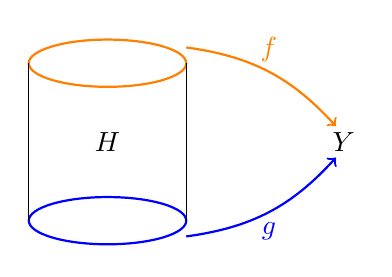
\begin{tikzpicture}
    \draw[blue, thick] (0, 0) ellipse(1 and 0.3);
    \draw[orange, thick] (0, 2) ellipse(1 and 0.3);

    \draw (-1, 0)--(-1, 2);
    \draw (1, 0)--(1, 2);

    \node at (3, 1) {$Y$};

    \path[->] (1, -0.2) edge [bend right=20, thick, blue] node [midway, below] {$g$} (2.9, 0.8);
    \path[->] (1, 2.2) edge [bend left=20, orange, thick] node [midway, above] {$f$} (2.9, 1.2);

    \node at (0, 1) {$H$};
  \end{tikzpicture}\end{center}

  Możemy do tego przyłożyć wiedzę o kompleksach, jeśli pod $X$ kryją się sympleksy. Wtedy mamy
  \begin{center}\begin{tikzpicture}[scale=1.5]
    \draw (0, 0) ellipse(1 and 0.3);
    \draw (0, 2) ellipse(1 and 0.3);

    \draw (-1, 0)--(-1, 2);
    \draw (1, 0)--(1, 2);

   % \draw[dashed] (-0.6, -0.1)--(-0.2, -0.15)--(-0.4, 0.1)--cycle;
   % \draw[dashed] (-0.4, 0.1)--(0, 0.15)--(-0.2, -0.15)--cycle;
   % \draw[dashed] (-0.2, -0.15)--(0.2, -0.15)--(0, 0.15)--cycle;
   % \draw[dashed] (0.2, -0.15)--(0.4 ,0.1)--(0, 0.15)--cycle;
   % \draw[dashed] (0.2, -0.15)--(0.4, 0.1)--(0.6, -0.1)--cycle;

    \draw[dashed] (-0.6, -0.1)--(-0.4, 0.1)--(-0.2, -0.15)--(0, 0.15)--(0.2, -0.15)--(0.4, 0.1)--(0.6, -0.1);
    \draw[dashed] (-0.4, 0.1)--(0, 0.15)--(0.4, 0.1);
    \draw (-0.6, -0.1)--(-0.2, -0.15)--(0.2, -0.15)--(0.6, -0.1);

    \draw (-0.6, 1.9)--(-0.2, 1.85)--(-0.4, 2.1)--cycle;
    \draw (-0.4, 2.1)--(0, 2.15)--(-0.2, 1.85)--cycle;
    \draw (-0.2, 1.85)--(0.2, 1.85)--(0, 2.15)--cycle;
    \draw (0.2, 1.85)--(0.4, 2.1)--(0, 2.15)--cycle;
    \draw(0.2, 1.85)--(0.4, 2.1)--(0.6, 1.9)--cycle;

    \draw(-0.6, -0.1)--(-0.6, 1.9);
    \draw(-0.2, -0.15)--(-0.2, 1.85);
    \draw(0.2, -0.15)--(0.2, 1.85);
    \draw(0.6, -0.1)--(0.6, 1.9);

    \draw[dashed] (-0.4, 0.1)--(-0.4, 2.1);
    \draw[dashed] (0, 0.1)--(0, 2.1);
    \draw[dashed] (0.4, 0.1)--(0.4, 2.1);

    \draw (2, 1.8)--(3, 2.2)--(1.8, 2.2)--cycle;
    \draw (2, -0.2)--(3, 0.2);
    \draw (2, -0.2)--(1.8, 0.2);
    \draw[dashed] (3, 0.2)--(1.8, 0.2);

    \draw (1.8, 0.2)--(1.8, 2.2);
    \draw (3, 0.2)--(3, 2.2);
    \draw (2, -0.2)--(2, 1.8);

    \node (HD) at (4, 1.5) {$H(\Delta)$};

    \path[->] (HD) edge [bend left=20] (2.4, 1);

    \node at (2.2, 2.1) {$\Delta$};
    \node at (2.5, -0.2) {$\partial$};

    \node at (4, 0.6) {$\substack{\partial H(\Delta)=f(\Delta)-g(\Delta)+\\+H(\partial\Delta)}$};
  \end{tikzpicture}\end{center}
\end{example}

\begin{fact}$ $

  \begin{enumerate}[label=(\alph*)]
    \item Relacja homotopijnej równoważności $\sim$ odwzorowań między ustalonymi kompleksami $A^*, B^*$ jest relacją równoważności
    \item Morfizmy $\sim 0$ tworzą "ideał", to znaczy 
      $$g, f\sim 0\implies f+g\sim 0$$
      $$(\forall\;k:B^*\to C^*,\; l:C^*\to A^*)\;f\sim 0\implies kf, fl\sim 0$$
    \item $f\sim g\implies H^i(f)=H^i(g)$
    \item Jeśli \begin{tikzcd}A^*\arrow[r, yshift=1mm, "f" above] & B^*\arrow[l, yshift=-1mm, "g" below]\end{tikzcd} są takie, że $fg\sim id_B$ oraz $gf\sim id_A$, to $f,g$ są qis oraz $H^i(f)=H^i(g)^{-1}$.
  \end{enumerate}
\end{fact}

\begin{proof}
  \begin{enumerate}[label=(\alph*)]
    \item Niech $f\overset{h}{\sim} g\overset{h'}{\sim} l$, wówczas $f\overset{h+h'}{\sim}l$. Wiemy więc, że 
      $$\begin{matrix}
        f-g = dh+hd\\ 
        g-l=dh'+h'd
      \end{matrix}$$
      dodając oba równania stronami, dostajemy
      $$f-l=(f-g)+(g-l)=(dh+hd)+(dh'+h'd)=(dh+dh')+(hd+h'd)=d(h+h')+(h+h')d.$$
    \item Jeśli $f, g\sim 0$ tak, że $f-0=dh+hd$ oraz $g-0=dh'+h'd$. Wtedy
      $$f+g=(f-0)+(g-0)=(dh+hd)+(dh'+h'd)=d(h+h')+(h+h')d.$$

      Pokażemy teraz, że dla $f\sim 0$ oraz dla dowolnego $k:B^*\to C^*$ mamy $kf\sim 0$. Rysując diagram
      \begin{center}
        \begin{tikzcd}[column sep=large, row sep=large, /tikz/column 1/.style={column sep=1mm}]
        A^*: & \bullet \arrow[d, "f" left] \arrow[r, dashed] & \bullet \tikzmark{A2} \arrow[d, "f" left] \arrow[r, dashed] \arrow[dl, "h" above] & \bullet \arrow[d, "f" left] \arrow[r, dashed] \arrow[dl, "h" above] & \bullet \arrow[d, "f" left] \\ 
        B^*: & \bullet \tikzmark{B1} \arrow[r, dashed] \arrow[d, "k" left] & \bullet \arrow[r, dashed, blue] \arrow[d, "k" left, red] & \bullet \arrow[r, dashed] \arrow[d, "k" left, blue] & \bullet \arrow[d, "k" left] \\ 
        C^*: & \bullet \tikzmark{C1} \arrow[r, dashed] & \bullet \arrow[r, dashed, red] & \bullet \arrow[r, dashed] & \bullet
        \end{tikzcd}
        \begin{tikzpicture}[remember picture, overlay]
          \draw[orange, ->, rounded corners] ([xshift=-2mm, yshift=-2mm]pic cs:A2) to ([xshift=2mm, yshift=2mm]pic cs:B1) node [right] {$k\circ h$} to ([xshift=2mm, yshift=2mm]pic cs:C1);
        \end{tikzpicture}
      \end{center} 
      Wiemy, że $f^i=h^{i+1}d+dh^i$, a dalej
      $$k^if^i=k^i(h^{i+1}d+dh^i)=k^i(h^{i+1}d)+k^i(dh^i)=(k^ih^{i+1})d+({\color{red}k^{i}d})h^i=(k^ih^{i})d+{\color{blue}d(k^{i-1}}h^{i})$$

    \item Wystarczy sprawdzić, że $f\sim 0\implies H^i(f)=0$. Niech $[a]\in H^i(f)$ zadaje klasę kohomologii, czyli $a\mapsto 0$ przez różniczkę $A^i\to A^{i+1}$.
      \begin{center}
        \begin{tikzcd}[/tikz/row 1/.style={row sep=1mm}, /tikz/row 3/.style={row sep=1mm}]
          & a\arrow[d, phantom, sloped, "\in"] \arrow[r, mapsto] & 0 \\ 
          A^{i-1} \arrow[r] \arrow[d] & A^i \arrow[r] \arrow[d] \arrow[dl, "h^i" above, blue] & A^{i+1} \arrow[d] \arrow[dl, "h^{i+1}" above, blue] \\ 
          B^{i-1} \arrow[r] & B^i \arrow[r] & B^{i+1} \\ 
          ? \arrow[r, dashed] & f^i(a)\arrow[r, mapsto] \arrow[u, phantom, sloped, "\in"] & 0
        \end{tikzcd}
      \end{center}
      Wiemy, że 
      $$f^i(a)=h^{i+1}\underbrace{d(a)}_{=0}+dh^i(a)=dh^i(a)$$
      czyli $h^i(a)$ jest w ramach $?$.
    \item Wynika z warunku c).
  \end{enumerate}
\end{proof}

\begin{fact}
  Niech $P^*\to X$ oraz $Q^*\to Y$ będą rezolwentami projektywnymi, a $f:X\to Y$ będzie morfizmem.
  \begin{enumerate}
    \item Istnieje morfizm rezolwent $R(f):P^*\to Q^*$ rozszerzający $f$ w sensie komutowania driagramu
      \begin{center}\begin{tikzcd}
        ... \arrow[r] & P^0\arrow[r, "\epsilon_x"]\arrow[d, "R(f)^0"] & X \arrow[d, "f"] \\ 
        ... \arrow[r] & Q^0 \arrow[r, "\epsilon_y"] & Y
      \end{tikzcd}\end{center}
      oraz diagramów "dalej na lewo".
    \item $R(f)$ jak wyżej jest jedyny z dokładnością do homotopii.
  \end{enumerate}
\end{fact}

\begin{conclusion}
  Gdy $Y=X$ i $f=id_X$, to mamy jedyne z dokładnością do homotopii przekształcenie między dwoma różnymi rezolwentami $X$.

  \begin{center}\begin{tikzcd}
    P^*\arrow[r]\arrow[d, "R" right, bend left=20] & X\arrow[d, "id"]\\ 
    Q^*\arrow[r]\arrow[u, bend left=20, "L" lef] & X
  \end{tikzcd}\end{center}
\end{conclusion}

\begin{proof}
  \begin{enumerate}[label=(\alph*)]
    \item Konstruujemy ten morfizm 
      \begin{center}\begin{tikzcd}
        P_0\arrow[r, "\epsilon_X"]\arrow[d, dashed] \arrow[dr, rounded corners, to path={([yshift=-4mm]\tikztostart) -| ([xshift=-5mm]\tikztotarget)}, blue] & X\arrow[r]\arrow[d, "f" right] & 0 \\ 
        Q_0\arrow[r, "\epsilon_Y" below] & Y \arrow[r] & 0
      \end{tikzcd}\end{center}
      Strzałka $P_0\to Q_0$ istnieje, ponieważ $P_0$ jest modułem projektywny, i $Q_0\to Y$ jest surjekcją. Czyli mamy diagram
      \begin{center}\begin{tikzcd}
        P_0\arrow[d, dashed]\arrow[dr] \\ 
        Q_0\arrow[r] & Y \arrow[r] & 0
      \end{tikzcd}\end{center}
  \end{enumerate}

  {\large\color{red}CHYBA WRÓCIĆ}
\end{proof}

\newpage

\section{27.11.23 : Klasa lokalizująca}

\begin{definition}[klasa lokalizująca]
  Klasa $S\subseteq Mor(\mathbf{B})$ spełnia następujące warunki
  \begin{enumerate}
    \item identyczność dla dowolnego obiektu należy do $S$ i dla dowolnych $s,t\in S$ które można składać $s\circ t\in S$
    \item Poniższe diagramy dopełniają się
      \begin{center}\begin{tikzcd}
        \bullet \arrow[r, dashed, green, "\in S"] \arrow[d, dashed] & \bullet\arrow[d] & & \bullet\arrow[r, green, "\in S"] \arrow[d] & \bullet\arrow[d, dashed]\\ 
        \bullet \arrow[r, green, "\in S" below] & \bullet & & \bullet\arrow[r, green, dashed, "\in S" below] & \bullet
      \end{tikzcd}\end{center}
      To znaczy, mając strzałki nieprzerywane znajdziemy strzałki przerywane tak, że odpowiednia strzałka jest z $S$ i powstałe diagramy komutują.
    \item Dla wszystkich \begin{tikzcd}X\arrow[r, yshift=1mm, "f"]\arrow[r, yshift=-1mm, "g" below] & Y\end{tikzcd} $(\exists\;s\in S)\;(sf=sg)\iff ((\exists\;t\in S)\;ft=gt)$.
  \end{enumerate}
\end{definition}

\newpage

\include{10:04-12-23.tex}
\newpage

\section{11.12.23 : Funktor Ext}
 
\begin{definition}[$Ext^i_{\mathbf{A}}(X, Y)$]
  Niech $\mathbf{A}$ będzie kategorią abelową. Rozważamy kategorie $Kom(\mathbf{A}), K(\mathbf{A}), D(\mathbf{A})$, które wszystkie mają te same obiekty.

  Niech $X\in\mathbf{A}$ będzie obiektem. Wtedy $\color{blue}X[-i]$ jest kompleksem, w który na $i$-tym miejscu stoi $X$:
  \begin{center}\begin{tikzcd}[row sep=tiny]
    ...\arrow[r] & 0\arrow[r] & X\arrow[r] & 0\arrow[r] & ... \\ 
                 & & i
  \end{tikzcd}\end{center}

  Dla $X,Y\in\ob\mathbf{A}$ definiujemy
  $$\color{blue}Ext_{\mathbf{A}}^i(X, Y)=Hom_{D(\mathbf{A})}(X[0], Y[i])$$
\end{definition}

Powyższe kategorie niekoniecznie są abelowe, ale na pewno są addytywne, więc na $Hom$ jak wyżej mamy zdefiniowaną operację dodawania.

Zauważmy, że
$$Hom_{D(\mathbf{A})}(X[0], Y[i])\cong Hom_{D(\mathbf{A})}(X[l], Y[i+l]).$$
możemy więc na $Ext$ zdefiniować mnożenie:
\begin{definition}[mnożenie $Ext$]
  $$Ext_{\mathbf{A}}^i(X, Y)\times Ext_{\mathbf{A}}^j(Y, Z)\xrightarrow{} Ext_{\mathbf{A}}^{i+j}(X, A)$$
  takie, że
  $$(X[0]\to Y[i])(Y[i]\to Z[j+i])\mapsto(X[0], Z[i+j])$$
\end{definition}

\subsection{Konstrukcja Yonedy}

Niech będzie dany ciąg dokładny
\begin{center}\begin{tikzcd}
  ...\arrow[r] & 0\arrow[r] & Y^{-i}\arrow[r] & K^{-i+1}\arrow[r] & ...\arrow[r] & K^0\arrow[r] & X\arrow[r] & 0\arrow[r] & ...
\end{tikzcd}\end{center}

Możemy wziąć fragment tego ciągu aż do $X$ i dopełnić go $0$. Dostajemy ciąg który nie jest już dokładny, więc dokładamy mu $X$ na dole, czyli tak naprawdę tworzymy odwzorowanie w kompleks $X[0]$ i drugie w kompleks $Y[i]$:
\begin{center}\begin{tikzcd}
  0\arrow[r] & Y\arrow[r]\arrow[d, "id"] & K^{-i+1}\arrow[r] & ... \arrow[r] & K^{0}\arrow[r]\arrow[d, "qis"] & 0\\ 
             & Y[i] & & & X[0]
\end{tikzcd}\end{center}
Tworzy się więc domek:
\begin{center}\begin{tikzcd}
  & K^*\arrow[dl, "qis" above left] \arrow[dr] \\ 
  X[0] & & Y[i] 
\end{tikzcd}\end{center}
Który nazywamy $Y(K^*)$ i jest on wtedy elementem $Ext_{\mathbf{A}}^i(X, Y)$.

\begin{example}
  \item $Ext^1$
    \begin{center}\begin{tikzcd}
      0\arrow[r] & Y \arrow[r] & K^0\arrow[r] & X\arrow[r] & 0 
    \end{tikzcd}\end{center}
  \item W kategorii przestrzeni wektorowych $Vect_K$ wszystkie $Ext=0$.
\end{example}

\begin{theorem}
  \begin{enumerate}[label=(\alph*)]
    \item Dla $i>0$ każdy element grupy $Ext_{\mathbf{A}}^i(X, Y)$ jest postaci $Y(K^*)$. To znaczy, że domki konstruowane wyżej są przydatne.
    \item $Ext^0(X, Y)=Hom_{\mathbf{A}}(X Y)$ (było tydzień temu)
    \item Dla $i<0$ $Ext^i(X, Y)=0$.
  \end{enumerate}
\end{theorem}

\begin{proof}
  \begin{enumerate}[label=(\alph*)]
    \item Zaczynamy od kompleksu $K^*$ i cały manewr będzie polegał na usunięciu wszystkiego, co nie jest między $-i$ a $0$. Rysujemy diagram
      \begin{center}\begin{tikzcd}
        & K^*\arrow[dl]\arrow[dr] \\ 
        X[0] & & Y[i]
      \end{tikzcd}\end{center}
    \item b
    \item Zaczynamy od diagramu dla $A^*\in Hom_{D(\mathbf{A})}(X[0], Y[i])$
      \begin{center}\begin{tikzcd}
        & A^*\arrow[dl, "s" above left]\arrow[dr, "f" above right] \\ 
        X[0] & & Y[i] \\ 
             & B^*\arrow[ul, "s'" above left, orange]\arrow[ur, "0", orange] \arrow[uu, "t", orange]
      \end{tikzcd}\end{center}
      pokażemy, że te pomarańczowe strzałki da się dorysować, by cały diagram komutował.

      Niech $B^*$ będzie kompleksem
      \begin{center}\begin{tikzcd}
        B^*=...\arrow[r] & A^{-i-2}\arrow[r] & \ker d^{-i-1}\arrow[r] & 0\arrow[r] & ... 
      \end{tikzcd}\end{center}
      czyli nad $Y$ ma zero, a nad $X$ ma bardzo podobny wygląd - na pewno homologie w $X$ się nie różnią od homologii w $X$ w kompleksie $A^*$.

      Nowy, zerowy, domek dominuje stary domek, więc ten stary też musiał być zerowy.
  \end{enumerate}

  {\large\color{red}CAŁY TEN DOWÓD TO POWINNAM NA ZDJĘCIA POPATRZEĆ JESZCZE RAZ}
\end{proof}

\subsection{Trójkąty wyróżnione}

\begin{definition}[wymiar homologiczny kategorii]
  Dla kategorii abelowej $\mathbf{A}$ definiujemy jej \buff{wymiar homologiczny} jako maksymalne $d$ takie, że 
  $$Ext_{\mathbf{A}}^d(X, y)\neq0 $$
  dla pewnych $X,Y\in\ob\mathbf{A}$. Oznaczamy $\color{blue}dh(\mathbf{A})=d$.
\end{definition}

\begin{example}
\item $dh(Vet_K)=0$
\item $dh(\mathbf{Ab})=1$
\item Dla pierścienia $R$ wymiar homologiczny (globalny) to $dh(R-mod)$. Na przykład pierścień wielomianów nad ciałem $\mathfrak{K}$, czyli $\mathfrak{K}[x_1,...,x_n]$, to ilość jego zmiennych $dh(\mathfrak{K}[x_1,..., x_n])=n$.
\end{example}

\begin{definition}[trójkąt wyróżniony]
  \buff{Trójkąt wyróżniony} [czasem nazywany dokladnym] w $K(\mathbf{A})$ lub w $D(\mathbf{A})$ to trójkąt izomorficzny z trójkątem postaci
  \begin{center}\begin{tikzcd}
    A^*\arrow[r, "f"] & B^*\arrow[r] & C(f)\arrow[r] & A^*[1]
  \end{tikzcd}\end{center}
\end{definition}

\begin{fact}\label{fakt 11.2}$ $\newline
  \begin{enumerate}[label=(\alph*)]
    \item $ $\newline
      \begin{center}\begin{tikzcd}
        X\arrow[r, "id"]\arrow[d] & X\arrow[r]\arrow[d] & 0\arrow[r]\arrow[d] & X[1] \\ 
        X\arrow[r, "id"] & X\arrow[r] & C(id_X)\arrow[r] & X[1] 
      \end{tikzcd}\end{center}
      i tutaj stożek $C(id_X)\cong 0$, bo $h(a^{i+1}, a^i)=(a^i, 0)$.
    \item Jeśli mamy trójkąt wyróżniony
      \begin{center}\begin{tikzcd}
        X\arrow[r, "u"] & Y \arrow[r] & Z\arrow[r] & X[1]
      \end{tikzcd}\end{center}
      to również 
      \begin{center}\begin{tikzcd}
        Y\arrow[r] & Z\arrow[r] & X[1]\arrow[r, "-u( 1 )"] & Y[1]
      \end{tikzcd}\end{center}
      też jest trójkątem wyróżnionym.
    \item Dla trójkątów wyróżnionych można uzupełniać diagramy, tzn. jeśli wiersze są trójkątami wyróżnionymi, to istnieje strzałka domykająca go:
      \begin{center}\begin{tikzcd}
        X\arrow[r]\arrow[d, "f"] & Y\arrow[r]\arrow[d, "g"] & Z\arrow[r]\arrow[d, dashed, blue, "\exists"] & X[1]\arrow[d, "f(1)"]\\ 
        X'\arrow[r] & Y'\arrow[r] & Z'\arrow[r] & X'[1]
      \end{tikzcd}\end{center}
  \end{enumerate}
\end{fact}

Te wszystkie własności pojawiają się w definicji kategorii striangulowanej. Poza nimi jest jeszcze jeden aksjomat, który jest bardzo skomplikowany, ale nie korzysta się z niego prawie nigdy.

\begin{lemma}
  W trójkącie wyróżnionym złożenie dwóch kolejnych odwzorowań jest zerowe jako morfizm w kategoriach $K(\mathbf{A})$ lub $D(\mathbf{A})$.
\end{lemma}

To znaczy, że samo w sobie niekoniecznie jest zerowe, ale jest homotopijne z odwzorowaniem zerowym.

\begin{proof}
  \begin{center}\begin{tikzcd}
    X\arrow[r, "id"] \arrow[d, "id"] & X\arrow[r]\arrow[d, "f"] & 0\arrow[r]\arrow[d, dashed, blue, "\exists"] & X[1]\arrow[d, "id"]\\ 
    X\arrow[r, "f"]\arrow[rr, orange, "0?" below, yshift=-2mm, bend right=10] & Y\arrow[r] & Z\arrow[r] & X[1]
  \end{tikzcd}\end{center}

  {\large\color{red}DOKOŃCZYĆ DIAGRAM}
\end{proof}

\begin{lemma}
  Niech $X\to Y\to Z\to X[1]$ będzie trójkątem wyróżnionym. Wtedy następujące ciąg są dokładne:
  \begin{center}\begin{tikzcd} 
    ...\arrow[r] & Hom(U, X[i]) \arrow[r] & Hom(U, Y[i]) \arrow[d, phantom, ""{coordinate, name=Z}] \arrow[r] & Hom(U, Z[i])\arrow[dll, rounded corners,
    to path={ -- ([xshift=2ex]\tikztostart.east)
|- (Z) [near end]\tikztonodes
-| ([xshift=-2ex]\tikztotarget.west)
-- (\tikztotarget)}
    ] \\ 
                 & Hom(U, X[i+1]) \arrow[r] & ...
  \end{tikzcd}\end{center}
  
  oraz

  \begin{center}\begin{tikzcd}
    ...\arrow[r] & Hom(Z[i], U)\arrow[r] & Hom(Y[i], U)\arrow[r] & Hom(X[i], U)
    \arrow[dll, rounded corners, 
to path={ -- ([xshift=2ex]\tikztostart.east)
|- (Z) [near end]\tikztonodes
-| ([xshift=-2ex]\tikztotarget.west)
-- (\tikztotarget)}
    ]\\ 
                 & Hom(Z[i-1], U)\arrow[r] & ...
  \end{tikzcd}\end{center}
\end{lemma}

Co jest ciekawe, to takie ciągi są dokładne niezależnie od tego, czy patrzymy w kategorii $K(\mathbf{A})$ czy $D(\mathbf{A})$.

\begin{proof}
  Ze względu na niezmienniczość tych trójkątów na przesunięcia (\ref{fakt 11.2} (b)), to wystarczy patrzeć na dokładność w jednym miejscu $X\xrightarrow{\alpha} Y\xrightarrow{\beta} Z$.

  Patrzymy więc na ciąg
  \begin{center}\begin{tikzcd}
    Hom(Z, U)\arrow[r, "\alpha^*"] & {\color{orange}Hom(Y, U)}\arrow[r, "\beta^*"] & Hom(X, U) 
  \end{tikzcd}\end{center}
  Zaczniemy od pokazania, że $\beta^*\circ\alpha^*=0$, ale to jest wprost z faktu, że 
  $$\alpha^*\beta^*=(\alpha\beta)^*=(0)^*=0$$
  ktore można narysować
  \begin{center}\begin{tikzcd}[column sep=large, row sep=large]
    X\arrow[r, "\alpha"]\arrow[dr, "\alpha^*\beta^*f" below left] & Y\arrow[r, "\beta"]\arrow[d, "\beta^*f"] & Z\arrow[dl, "f" below right]\\ 
                                                       & W
  \end{tikzcd}\end{center}
  Dalej chcemy sprawdzić, czy $\ker\alpha^*=\img\beta^*$? Najpierw zauważmy, że jeśli $f\in\ker\alpha^*$, to wówczas
  \begin{center}\begin{tikzcd}
    X\arrow[r, "\alpha"]\arrow[dr, "0" below left] & Y\arrow[d, "f"] \\ 
                                                   & U
  \end{tikzcd}\end{center}
  komutuje. Czyli rysując już docelowy diagram, mamy:
  \begin{center}\begin{tikzcd}
    X\arrow[r, "\alpha"]\arrow[d, "0", orange] & Y\arrow[r, "\beta"]\arrow[d, "f", orange] & Z\arrow[r]\arrow[d, dashed, "\exists", blue] & X[1]\arrow[d, "0(1)", orange] \\ 
    0\arrow[r] & U\arrow[r, "id"] & U\arrow[r] & 0
  \end{tikzcd}\end{center}
  Niebieskie odwzorowanie zamyka diagram, stąd $id$ między $U$. Czyli 
  $$g\beta=f\implies \beta^* g=f$$
\end{proof}

\begin{conclusion}
  Niech 
  \begin{center}\begin{tikzcd}
    0\arrow[r] & A\arrow[r] & B\arrow[r] & C\arrow[r] & 0
  \end{tikzcd}\end{center}
  będzie krótkim ciągiem dokładnym w $\mathbf{A}$. Prowadzi on do trójkąta wyróżnionego $A\to B\to C\to A[1]$ w kategorii $D(\mathbf{A})$ (ćwiczenia).

  Dzięki temu można pisać długie ciągi dokładne dla $U\in\ob\mathbf{A}$:
  \begin{center}\begin{tikzcd}
    ...\arrow[r] & Ext^i(C, U)\arrow[r] & Ext^i(B, U)\arrow[r] & Ext^i(A, U)\arrow[r] & Ext^{i+1}(C, U)\arrow[r] &... 
  \end{tikzcd}\end{center}

  i tak samo dla drugiej funktorialności:
  \begin{center}\begin{tikzcd}
    ...\arrow[r] & Ext^i(U,A)\arrow[r] & Ext^i(U, B)\arrow[r] & Ext^i(U, C)\arrow[r] & Ext^{i+1}(U, A)\arrow[r] &... 
  \end{tikzcd}\end{center}
\end{conclusion}

\begin{fact}
  Jeśli $dh(\mathbf{A})=0$, to każdy krótki ciąg dokładny W $\mathbf{A}$
  \begin{center}\begin{tikzcd}
    0\arrow[r] & A\arrow[r] & B\arrow[r] & C\arrow[r] & 0
  \end{tikzcd}\end{center}
  rozszczepia się, tzn. istnieje
  \begin{center}\begin{tikzcd}
    0\arrow[r] & A\arrow[r, "\alpha"] & B\arrow[r, "\beta", yshift=1mm] & C\arrow[r]\arrow[l, yshift=-1mm, "\exists \gamma"] & 0
  \end{tikzcd}\end{center}
  takie, że $\beta\gamma=Id_C$. Stąd
  \begin{center}\begin{tikzcd}
    0\arrow[r] & A\arrow[r]\arrow[dr] & A\oplus C\arrow[r] & C\arrow[r] & 0\\ 
               &            & B\arrow[ur]\arrow[u, phantom, sloped, "\cong"]
  \end{tikzcd}\end{center}
\end{fact}

\begin{proof}
  Niech \begin{tikzcd}0\arrow[r] & A\arrow[r] & B\arrow[r] & C\arrow[r] & 0\end{tikzcd} będzie ciągiem dokładnym. Wtedy dla $U=A$ mamy
  \begin{center}\begin{tikzcd}
    0\arrow[r] & Ext^0(C, A)\arrow[r] & Ext^0(B, A)\arrow[r] & Ext^0(A, A) \arrow[r] & Ext^1(C, A) \arrow[r] &...
\\ 
               & Hom(C, A)\arrow[u, phantom, sloped, "="]\arrow[r] & Hom(B, A)\arrow[r] & Hom(A, A)\arrow[r] & 0\arrow[u, phantom, sloped, "="]\\ 
               & & \delta\arrow[u, phantom, sloped, "\in"]\arrow[r, mapsto] & id_A\arrow[u, phantom, sloped, "\in"]
  \end{tikzcd}\end{center}
  Stąd mamy $\ker \delta\xrightarrow{\beta} C$ i $\gamma:C\to \ker\delta$ i wtedy $\delta\alpha=id_A$ i całość rozszczepia się.
\end{proof}

\begin{conclusion}
  $dh(\mathbf{Ab})\geq 1$, bo $0\to \Z\to \Z\to \Z/2\to 0$ nie rozszczepia się.
\end{conclusion}

\subsection{Warianty kategorii pochodnej}

\begin{enumerate}
  \item $D^+(\mathbf{A})$ - podkategoria rozpinana przez kompleksy zerujące się na lewo od pewnego indeksu ($A^i=0$ dla $i<<0$)
  \item $D^-(\mathbf{A})$ - podkategoria rozpinana przez kompleksy zerujące się na prawo od pewnego indeksu ($A^i=0$ dla $i>>0$)
  \item $D^b(\mathbf{A})$ - podkategoria rozpinana przez kompleksy "ograniczone" ($A^i=0$ dla $|i|>>0$)
\end{enumerate}

\begin{definition}
  W kategorii $\mathbf{A}$ jest \acc{wystarczająco dużo obiektów injektywnych}, jeśli każdy obiekt wkłada się w pewien obiekt injektywny. Analogicznie mówimy, że w $\mathbf{A}$ jest \acc{dostatecznie dużo obiektów projektwynych}, jeśli każdy obiekt jest ilorazem (istnieje surjekcja) obiektu projektywnego.
\end{definition}

\begin{theorem}
  Jeśli w $\mathbf{A}$ jest dostatecznie dużo obiektów injektywnych, to naturalny funktor 
  $K^+(I)\to D^+(\mathbf{A})$ jest równoważnością kategorii.
\end{theorem}

$I$ jest klasą wszystkich injektywnych obiektów kategorii $\mathbf{A}$. Z kolei $K^+(I)$ to wszystkie kompleksy o obiektach injektywnych z dokładnością do homotopii. Analogicznie, $K^-(P)$ będzie zawierało wszystkie kompleksy na obiektach projektywnych z dokładnością do homotopii.

\begin{lemma}\label{lemat skladanie z qis}
  W $K^(\mathbf{A})$ niech $f:X\to Y$ będzie qis. Załóżmy, że mamy kompleks obiektów injektywnych $I^*$. Wtedy
  $$Hom_{K(\mathbf{A})}(Y^*, I^*)\xrightarrow{-\circ s}Hom_{K(\mathbf{A})}(X^*, I^*)$$
  jest izomorfizmem. 
\end{lemma}

\begin{proof}
  W przyszłym tygodniu
\end{proof}

\begin{conclusion}
  Jeśli $A^*$ oraz $I^*$ są kompleksami zaczynającymi się od pewnego miejsca ($\in Kom^+(\mathbf{A})$), a $I^*$ jest injektywny, to wtedy
  $$Hom_{K(\mathbf{A})}(A^*, I^*)\cong Hom_{D(\mathbf{A})}(A^*, I^*)$$
\end{conclusion}

\begin{proof}
  \begin{center}\begin{tikzcd}
    & B^*\arrow[dl, "qis=s" above left] \arrow[dr, "f"] \\ 
    A^*\arrow[rr, "f", dashed, blue] & & I^* 
  \end{tikzcd}\end{center}

  Zaczniemy od pokazania, że $Hom_{K(\mathbf{A})}(A^*, I^*)\to Hom_{D(\mathbf{A})}(A^*, I^*)$ jest epimorfizmem
  \begin{center}\begin{tikzcd}
    & B^*\arrow[dr, "s"] \arrow[dl, "f"] \arrow[dd, "s"] \\ 
    A^* & & I^* \\  
    & A^*\arrow[ul, "id"] \arrow[ur, "f'"]
  \end{tikzcd}\end{center}
  
  Natomiast monomorfizm tej strzałki wynika z tego, że 
  \begin{center}\begin{tikzcd}
    & & B^*\arrow[dl, "s"]\arrow[dr, "s"]\\ 
    & A^*\arrow[dl, "id"]\arrow[drrr, "f"] &   & A^*\arrow[dr, "g"]\arrow[dlll, "id"] \\ 
    A^* & & & & I^* 
  \end{tikzcd}\end{center}
  Chcemy z tego wywnioskować, że skoro $fs\cong gs$, to $f$ jest homotopijne z $g$ i używamy do tego lemat \ref{lemat skladanie z qis}.
\end{proof}

\newpage

\include{12:18-12-23.tex}
\newpage 
 
\section{08.01.24 : }

\begin{center}\begin{tikzcd}
  K^+(I_\mathbf{A})\arrow[r]\arrow[dr, yshift=1mm, "\iota"] & K^+(\mathbf{A})\arrow[r, "K(F)"]\arrow[d] & K^+(\mathbf{B})\arrow[d]\\ 
                                                            & D^+(\mathbf{A})\arrow[ul, "\iota^{-1}", yshift=-1mm] & D^+(\mathbf{B})
\end{tikzcd}\end{center}

\begin{definition}
  Dla dowolnego $A\in\ob\mathbf{A}$ definiujemy
  $$R^iF(A):=H^i(RF(A[0]))$$
\end{definition}

\begin{fact}
  Jeśli $F$ jest lewo dokładny, i $0\to A\to B\to C\to 0$ jest dokładny w $\mathbf{A}$, to również
  \begin{center}\begin{tikzcd}
    0\arrow[r] & F(A)\arrow[r] & F(B)\arrow[r] & F(C)\arrow[r] R^1F(A)\arrow[r] R^1F(B)\arrow[r] & R^1F(C)\arrow[r] & R^2F(A)\arrow[r] & ...
    \end{tikzcd}\end{center}
    jest ciągiem dokładnym.
\end{fact}

\begin{fact}
  $$Ext_\mathbf{A}^i(A,-)=R^iHom(A, -)$$
\end{fact}

\begin{proof}
  Policzmy $(R^iHom(A, -))(B)$ dla dowolnego $B\in \mathbf{A}$. Mamy rezolwentę injektywną
  $$B\to I^0\to I^1\to I^2\to ...$$
  dostajemy wówczas
  \begin{center}\begin{tikzcd}
    ...\arrow[r] & 0\arrow[r] & Hom(A, I^0)\arrow[r] & Hom(A, I^1)\arrow[r] & Hom(A, I^2)
  \end{tikzcd}\end{center}
  Szukana grupa (obiekt) to 
  $$\ker d:\frac{Hom(A, I^i)\to Hom(A, I^{i+1})}{\img d:Hom(A, I^{i+1})\to Hom(A, I^i)}/$$
  Dowolna strzałka $Hom(A, I^i)\ni f:A\to I^i$ jest w $\ker d$ $\iff$ odwzorowanie
  \begin{center}\begin{tikzcd}
    ...\arrow[r] & 0\arrow[r]\arrow[d, "0"] & A\arrow[r]\arrow[d, "f"] & 0\arrow[r]\arrow[d, "0"] & 0\arrow[r]\arrow[d, "0"] & ...\\
    ...\arrow[r] & I^{i-1} \arrow[r] & I^i\arrow[r] & I^{i+1}\arrow[r] & I^{i+2}\arrow[r] & ...
  \end{tikzcd}\end{center}
  jest morfizmem kompleksów
  $$\ker d:\underbrace{Hom(A, I^i)}_{=Hom_{Kom\mathbf{A}}(A[i], I^*)}\to Hom(A, I^{i+1})$$

  Taka sama strzałka $f:A\to I^i$ jest w obrazie $\img d$ $\iff$ odwzorowanie kompleksów
  \begin{center}\begin{tikzcd}
    0\arrow[r]\arrow[d] & A\arrow[r]\arrow[d, "f"]\arrow[dl, green, "h"] & 0\arrow[d]\\ 
    I^{i-1}\arrow[r] & I^i\arrow[r] & I^{i+1}
  \end{tikzcd}\end{center}
  jest homotopijne z zerem.

  Zatem dostajemy
  $$H^i(Hom(A, I^*))=Hom_{K^+(\mathbf{A})}(A[i], I^*)$$
  ale ponieważ $I^*$ jest injektywny, to
  $$Hom_{K^+(\mathbf{A})}(A[i], I^*)=Hom_{D^+(\mathbf{A})}(A[i], I^*)$$
  ale przecież w  $D^+\mathbf{A}$ mamy $I^*\cong B[0]$, więc
  $$Hom_{D^+\mathbf{A}}(A[i], I^*)=Hom_{D^+\mathbf{A}}(A[i], B[0])=Ext^i_{\mathbf{A}}(A, B).$$
\end{proof}

\begin{fact}
  \begin{enumerate}
    \item $RF$ jest dokładny.
    \item $\exists$ naturalne przekształcenie $\epsilon_F:Q_B\circ K(F)\implies RF\circ Q_A$
    \item Jeśli $G:D^+\mathbf{A}\to D^+\mathbf{B}$ jest dokładny i dopuszcza naturalne przekształcenie $\epsilon_G:Q_B\circ K(F)\implies G\circ Q_A$ analogiczne jak wyżej, to istnieje naturalne przekształcenie $\eta:RF\to G$, które zamyka diagram
      \begin{center}\begin{tikzcd}
        & RF\circ Q_A\arrow[dd, "\eta"]\\
        Q_B\circ K(F)\arrow[ur, "\epsilon_F"]\arrow[dr, "\epsilon_G"]\\ 
        & G\circ Q_A
      \end{tikzcd}\end{center}
  \end{enumerate}
\end{fact}

\begin{proof}
  \begin{enumerate}
    \item Mając dany trójkąt wyróżniony \begin{tikzcd} A^*\arrow[r, "f"] & B^*\arrow[r] & C(f)\arrow[r] & A^*[1] \end{tikzcd} produkujemy stożek w sposób funktorialny
      \begin{center}\begin{tikzcd}
        F(A^*)\arrow[r, "F(f)"] & F(B^*)\arrow[r] & F(C(f))\arrow[r, "="] & C(F(f))
      \end{tikzcd}\end{center}

      Stąd $K(F)$ i $Q_B$ są dokładne. Ponieważ $RF=Q_B\circ K(F)\circ \iota^{-1}$, to wystarczy pokazać, że $\iota^{-1}$ jest dokładna.

      Bierzemy więc trójkąt wyróżniony w $D^+\mathbf{A}$, zaznaczony na zielono. Naszym celem będzie pokazać, że druga od góry linijka jest trójkątem wyróżninym
      \begin{center}\begin{tikzcd}
        \iota^{-1}A\arrow[r, "g"]\arrow[d, "="] & \iota^{-1} B\arrow[r]\arrow[d, "="] & C(g) \arrow[r] & \iota^{i-1}A[1]\arrow[d, "="] & \Delta\text{ w }K^+(I_\mathbf{A})\\

        \iota^{-1}A\arrow[r, "g"]\arrow[d, "\cong"] &\iota^{-1} B\arrow[r]\arrow[d, "\cong"] & \iota^{-1}C\arrow[r]\arrow[d, "\cong"] & \iota^{-1}A[1]\arrow[d, "\cong"] & \text{trójkąt w }K^+(I_\mathbf{A})\\
        \color{green}A\arrow[r, green] \arrow[d, "\cong"] &\color{green} B\arrow[r, green]\arrow[d, "\cong"] & \color{green} C\arrow[r, green] \arrow[d, "\cong"] & \color{green} A[1]\arrow[d, "\cong"] & \text{wyjściowy }\Delta\\ 
        A'\arrow[r]\arrow[uuu, bend left=20, orange] & B'\arrow[r]\arrow[uuu, bend left=20, orange] & C(f)\arrow[r]\arrow[uuu, dashed, orange, bend left=20, "\exists\phi" left] & A'[1]\arrow[uuu, bend right=20, orange] & \Delta\text{ w }Kom^+(\mathbf{A})
      \end{tikzcd}\end{center}
      pomarańczowa strzałka istnieje, ponieważ pomarańczowe strzałki to izomorfizmy między wyrazami trójkątów wyróżnionych -> musi się więc domknąć do pełnego odwzorowania między tymi trójkątami. Pokażemy teraż, że $\phi:C(f)\to C(g)$ jest qis. Rozważamy ciągi dokładne trójkątów:
      \begin{center}\begin{tikzcd}
        H^i(\iota^{-1}A)\arrow[r] & Hom^i(\iota^{-1}B)\arrow[r] & H^i(C(g))\arrow[r] & H^{i+1}(\iota^{-1}A)\arrow[r] & Hom^{i+1}(\iota^{-1}B)\\ 
        H^i(A')\arrow[u, "\cong"]\arrow[r] & H^i(B')\arrow[u, "\cong"]\arrow[r] & H^i(C(f))\arrow[u,dashed]\arrow[r] & H^{i+1}(A')\arrow[u, "\cong"]\arrow[r] & H^{i+1}(B')\arrow[u, "\cong"]
      \end{tikzcd}\end{center}
      z lematu o $5$ izomorfizmach wiemy, że strzałka z $H^i(C(f))$ jest izomorfizmem, czyli w rzeczy samej, $\phi$ jest qis.

      Mamy więc z tego odwzorowanie trójkąta z drugiej linii do trójkąta z 1 linii i to odwzorowanie jest izomorfizmem w $D^+(\mathbf{A})$. Ponieważ 1 i 2 linia składają się z obiektów injektywnych, to izomorfizm ten realizuje się w $K^+(\mathbf{A})$.

    \item Mamy diagram
      \begin{center}\begin{tikzcd}[column sep=large, row sep=large]
        K^+\mathbf{A}\arrow[r, "K(F)"]\arrow[d, "Q_A" left] & K^+\mathbf{B}\arrow[d, "Q_B"]\arrow[dl, "\varepsilon_F"]\\ 
        D^+\mathbf{A}\arrow[r, "RF" below] & D^+\mathbf{B}
      \end{tikzcd}\end{center}
      i drugi
      \begin{center}\begin{tikzcd}
        & A^*\arrow[r] \arrow[d] & F(A^*)\arrow[d]\\ 
        & A^*\arrow[dl, "\mu(A^*)" above left]\arrow[dr] & \arrow[dd, bend left=40, "F(\mu(A^*))"] F(A^*)\\ 
        I^* & & RF(A^*)\arrow[d, "\cong"]\\ 
            & & F(I^*)
      \end{tikzcd}\end{center}
    \item 
      \begin{center}\begin{tikzcd}
        K^+\mathbf{A}\arrow[d] \arrow[r, "K(F)"] & K^+\mathbf{B} \arrow[d] \\ 
        D^+\mathbf{A} \arrow[r, bend left=20, "RF" above]\arrow[r, bend right=20, "G" below] & D^+\mathbf{B}
      \end{tikzcd}\end{center}
      {\large\color{red}ZDJĘCIE}
  \end{enumerate}
\end{proof}

Jeśli $A, B$ są $R$-modułami, to $Tor(A, B)$ liczymy biorąc rezolwentę projektywną
$$...\to P_1\to P_0\to B$$ 
tensorujemy ją z $A$ i dostajemy
$$...\to A\otimes P_2\to A\otimes P_1\to A\otimes P_0\to 0$$
Wtedy kohomologie tego nowego kompleksu to tory: $H^i=Tor_i(A, B)$
  
\begin{theorem}
  Niech $\mathbf{A},\mathbf{B}$ będą kategoriami abelowymi takimi, że w $\mathbf{A}$ jest dostatecznie dużo oniektów injektywnych $I_\mathbf{A}$. Niech 
  $$F:\mathbf{A}\to \mathbf{B}$$
  będzie addytywnym i lewo-dokładnym funktorem. Niech $I_F$ będzie klasą obiektów $F$-acyklicznych. To znaczy takich $A\in\ob\mathbf{A}$, dla których $R^iF(A)=0$ dla $i>0$. Wtenczas
  \begin{enumerate} 
    \item $I_A\subseteq I_F$
    \item jeśli $A^*\in Kom^+\mathbf{A}$ jest dokładny oraz $A^i\in I_F$, to wówczas $F(A^*)$ też jest dokładny
    \item jeśli $A\to A^*$ jest rezolwentą $F$-acykliczną, to 
      $$RF(A[0])=RF(A^*)=F(A^*)$$
      a co więcej
      $$R^iF(A)=H^i(F(A^*)).$$
  \end{enumerate}
\end{theorem}

\begin{proof}
  \begin{enumerate}
    \item Niech $I\in I_A$ i chcemy sprawdzić, że wyższe pochodne $R^iF(I)=0$. Rozważamy rezolwentę injektywną $I$:
      \begin{center}\begin{tikzcd}
        I\arrow[r] \arrow[d, "F"] & I\arrow[r] & 0\arrow[r] & 0\arrow[r] & ... \\ 
        0\arrow[r] & F(I)\arrow[r] & 0\arrow[r] & 0 \arrow[r] & ...
      \end{tikzcd}\end{center}
      czyli $H^*$ to $0\quad F(I)=R^0F(I) \quad 0\quad 0=R^2F(I)\quad ...$.
    \item  Bez straty ogólności rozważmy
      $$0\to A^0\to A^1\to A^2\to....$$
      Niech $B^i=\img(d:A^{i-1}\to A^i)$. Z dokładności $A^*$ wynika dokładność ciągu
      $$0\to A^0\to B^1\to 0.$$
      W następnym korku możemy popatrzeć na włożenie $B^1\to A^2$, którego iloraz przez jądro jest dokładnie równe $B^2$. Kontynuując ten tok myślenia dostajemy cały zestaw ciągów dokłądnych
      $$0\to B^1\to A^1\to B^2\to 0$$
      $$0\to B^2\to A^2\to B^3\to 0$$
      $$...$$
      Czyli $B^1\cong A^0$ jest $F$-acykliczny. Z zestawu ciągów dokładnych dostajemy ciąg indukowany przez $F$
      \begin{center}\begin{tikzcd}
        0\arrow[r] & FB^1\arrow[r] & FA^1\arrow[r] & FB^2\arrow[r] & R^1F(B^1)\arrow[r] & R^1F(A^1)\arrow[r] & R^1F(B^2)\arrow[r] & R^2F(B^1)\arrow[r] & ...\\ 
                   & & & & 0\arrow[u, phantom, sloped, "="] & 0\arrow[u,phantom,sloped,"="] & 0 & 0
      \end{tikzcd}\end{center}

      \begin{center}\begin{tikzcd}
        & & 0 & & 0\\ 
        & & & B^k \\
        & & A^{k-1} & & A^k
      \end{tikzcd}\end{center}
      {\color{red}ZDJĘCIE}
    \item Użyjemy do tego punktu rezolwenty C-E z poprzedniego wykładu.
      Odwzorowanie $A[0]\to A^*$ jest qis, czyli jest izomorfizmem w $D^+\mathbf{A}$. Czyli $RF(A[0])\cong RF(A^*)$, w szczególności $R^iF(A)\cong H^i(RF(A^*))$.
      {\large\color{red}ZDJĘCIE BO NIE PRZEJDZIE RYSOWANIE TEGO}
  \end{enumerate}
\end{proof}

\begin{theorem}[o składaniu funktorów]
  Załóżmy, że są trzy kategorie abelowe $\mathbf{A},\mathbf{B},\mathbf{C}$ mające dostatecznie dużo obiektów injektywnych i dwa funktory $F:\mathbf{A}\to \mathbf{B}$ i $G:\mathbf{B}\to \mathbf{C}$, które są addytywne i lewo-dokładne. Załóżmy ponadto, że $G(I_\mathbf{A})\subseteq I_F$. Wtedy
  $$R(F\circ G)\cong RF\circ RG$$
  funktor pochodny złożenia jest izomorficzny ze złożeniem funktorów pochodnych.
\end{theorem}

\begin{proof}
  Z uniwersalności dostajemy $\varepsilon:R(F\circ G)\to RF\circ RG$.
  \begin{center}\begin{tikzcd}
    K^+\mathbf{C}\arrow[d]\arrow[dr, "\varepsilon_F"] & K^+\mathbf{B}\arrow[l]\arrow[d]\arrow[dr, "\varepsilon_G"] & K^+\mathbf{A}\arrow[l]\arrow[d] \\ 
    D^+\mathbf{C} & \arrow[l, "RF"] D^+\mathbf{B} & \arrow[l, "RG"] D^+\mathbf{A}
  \end{tikzcd}\end{center}
  {\large\color{red}ZDJĘCIE, BO COŚ SIĘ POPSUŁO}
\end{proof}



\end{document}
